
%%\documentclass[12pt,preprint]{aastex}

%% manuscript produces a one-column, double-spaced document:

%% \documentclass[10pt,manuscript]{aastex}

%% preprint2 produces a double-column, single-spaced document:
\documentclass[preprint2,apjl,numberedappendix,twocolappendix,appendixfloats]{emulateapj}
%% \documentclass[preprint2,iop]{aastex}

%% \documentclass[preprint2,longabstract]{aastex}

%% \usepackage{ccaption}
%% \captionstyle{\raggedright}
\usepackage[caption=false]{subfig}
\usepackage{amsmath}
\usepackage{footnote}
\bibpunct{(}{)}{;}{a}{}{,} 
\captionsetup{belowskip=12pt,aboveskip=4pt}
\setlength{\textfloatsep}{10pt plus 1.0pt minus 2.0pt}
\newcommand{\dif}{\mathrm{d}}
%% \renewcommand*{\thefootnote}{\fnsymbol{footnote}}

\def\nar{{New~A~Rev.}}          % New Astronomy Review
\def\pasa{{PASA}}               % Publications of the Astron. Soc. of Australia

%% \bibliographystyle{mn2e}
%% \bibliographystyle{apj}

\shorttitle{MWA Observations of Wide-field Effects in EoR Power Spectra}
\shortauthors{Thyagarajan et~al.}

\def\ASU{\altaffilmark{1}}
\def\ASUtxt{\altaffiltext{1}{Arizona State University, School of Earth and Space Exploration, Tempe, AZ 85287, USA}}

\def\myemail{\altaffilmark{*}}
\def\myemailtxt{\altaffiltext{*}{e-mail: t\_nithyanandan@asu.edu}}

\def\UW{\altaffilmark{2}}
\def\UWtxt{\altaffiltext{2}{University of Washington, Department of Physics, Seattle, WA 98195, USA}}

\def\SKASA{\altaffilmark{3}}
\def\SKASAtxt{\altaffiltext{3}{Square Kilometre Array South Africa (SKA SA), Park Road, Pinelands 7405, South Africa}}

\def\RU{\altaffilmark{4}}
\def\RUtxt{\altaffiltext{4}{Department of Physics and Electronics, Rhodes University, Grahamstown 6140, South Africa}}

\def\CfA{\altaffilmark{5}}
\def\CfAtxt{\altaffiltext{5}{Harvard-Smithsonian Center for Astrophysics, Cambridge, MA 02138, USA}}

\def\ANU{\altaffilmark{6}}
\def\ANUtxt{\altaffiltext{6}{Australian National University, Research School of Astronomy and Astrophysics, Canberra, ACT 2611, Australia}}

\def\CAASTRO{\altaffilmark{7}}
\def\CAASTROtxt{\altaffiltext{7}{ARC Centre of Excellence for All-sky Astrophysics (CAASTRO)}}

\def\Haystack{\altaffilmark{8}}
\def\Haystacktxt{\altaffiltext{8}{MIT Haystack Observatory, Westford, MA 01886, USA}}

\def\RRI{\altaffilmark{9}}
\def\RRItxt{\altaffiltext{9}{Raman Research Institute, Bangalore 560080, India}}

\def\MIT{\altaffilmark{10}}
\def\MITtxt{\altaffiltext{10}{MIT Kavli Institute for Astrophysics and Space Research, Cambridge, MA 02139, USA}}

\def\Curtin{\altaffilmark{11}}
\def\Curtintxt{\altaffiltext{11}{International Centre for Radio Astronomy Research, Curtin University, Perth, WA 6845, Australia}}

\def\Victoria{\altaffilmark{12}}
\def\Victoriatxt{\altaffiltext{12}{Victoria University of Wellington, School of Chemical \& Physical Sciences, Wellington 6140, New Zealand}}

\def\UWisc{\altaffilmark{13}}
\def\UWisctxt{\altaffiltext{13}{University of Wisconsin--Milwaukee, Department of Physics, Milwaukee, WI 53201, USA}}

\def\UMelbourne{\altaffilmark{14}}
\def\UMelbournetxt{\altaffiltext{14}{The University of Melbourne, School of Physics, Parkville, VIC 3010, Australia}}

\def\USydney{\altaffilmark{15}}
\def\USydneytxt{\altaffiltext{15}{The University of Sydney, Sydney Institute for Astronomy, School of Physics, NSW 2006, Australia}}

\def\CASS{\altaffilmark{16}}
\def\CASStxt{\altaffiltext{16}{CSIRO Astronomy and Space Science (CASS), PO Box 76, Epping, NSW 1710, Australia}}

\def\Tata{\altaffilmark{17}}
\def\Tatatxt{\altaffiltext{17}{National Centre for Radio Astrophysics, Tata Institute for Fundamental Research, Pune 411007, India}}

% \def\NRAO{\altaffilmark{19}}
% \def\NRAOtxt{\altaffiltext{19}{National Radio Astronomy Observatory, Charlottesville and Greenbank, USA}}

% \def\UMichigan{\altaffilmark{13}}
% \def\UMichigantxt{\altaffiltext{13}{University of Michigan, Department of Atmospheric, Oceanic and Space Sciences, Ann Arbor, MI 48109, USA}}

% \def\UWA{\altaffilmark{20}}
% \def\UWAtxt{\altaffiltext{20}{International Centre for Radio Astronomy Research, University of Western Australia, Crawley, WA 6009, Australia}}

%% \definenote[thanks][conversion=set 2]

\begin{document}

\title{Confirmation of Wide-Field Signatures in Redshifted 21~cm Power Spectra
using Murchison Widefield Array Observations}

%% Use \author, \affil, and the \and command to format
%% author and affiliation information.
%% Note that \email has replaced the old \authoremail command
%% from AASTeX v4.0. You can use \email to mark an email address
%% anywhere in the paper, not just in the front matter.
%% As in the title, use \\ to force line breaks.

%% Author list
\author{
%% Lead Authors
Nithyanandan~Thyagarajan\ASU\myemail,
Daniel~C.~Jacobs\ASU,
Judd~D.~Bowman\ASU,
N.~Barry\UW,
A.~P.~Beardsley\UW,
G.~Bernardi\SKASA$^,$\RU$^,$\CfA,
F.~Briggs\ANU$^,$\CAASTRO,
R.~J.~Cappallo\Haystack, 
P.~Carroll\UW,
% B.~E.~Corey\Haystack, 
A.~A.~Deshpande\RRI, 
A.~de~Oliveira-Costa\MIT,
Joshua~S.~Dillon\MIT,
% D.~Emrich\Curtin,
% B.~M.~Gaensler\USydney$^,$\CAASTRO, 
A.~Ewall-Wice\MIT,
L.~Feng\MIT,
% R.~Goeke\MIT,
L.~J.~Greenhill\CfA,
B.~J.~Hazelton\UW,
L.~Hernquist\CfA, 
J.~N.~Hewitt\MIT,
N.~Hurley-Walker\Curtin,
M.~Johnston-Hollitt\Victoria,
D.~L.~Kaplan\UWisc, 
% J.~C.~Kasper\UMichigan$^,$\CfA, 
Han-Seek~Kim\UMelbourne$^,$\CAASTRO,
P.~Kittiwisit\ASU,
% E.~Kratzenberg\Haystack, 
E.~Lenc\USydney$^,$\CAASTRO,
J.~Line\UMelbourne$^,$\CAASTRO,
A.~Loeb\CfA,
C.~J.~Lonsdale\Haystack, 
% M.~J.~Lynch\Curtin, 
B.~McKinley\UMelbourne$^,$\CAASTRO,
S.~R.~McWhirter\Haystack,
D.~A.~Mitchell\CASS$^,$\CAASTRO, 
M.~F.~Morales\UW, 
E.~Morgan\MIT, 
A.~R.~Neben\MIT,
D.~Oberoi\Tata, 
A.~R.~Offringa\ANU$^,$\CAASTRO, 
S.~M.~Ord\Curtin$^,$\CAASTRO,
Sourabh~Paul\RRI,
B.~Pindor\UMelbourne$^,$\CAASTRO,
J.~C.~Pober\UW,
T.~Prabu\RRI, 
P.~Procopio\UMelbourne$^,$\CAASTRO,
J.~Riding\UMelbourne$^,$\CAASTRO,
% A.~E.~E.~Rogers\Haystack, 
% A.~Roshi\NRAO, 
N.~Udaya~Shankar\RRI, 
Shiv~K.~Sethi\RRI,
K.~S.~Srivani\RRI, 
R.~Subrahmanyan\RRI$^,$\CAASTRO, 
I.~S.~Sullivan\UW,
M.~Tegmark\MIT,
S.~J.~Tingay\Curtin$^,$\CAASTRO, 
C.~M.~Trott\Curtin$^,$\CAASTRO,
% M.~Waterson\Curtin$^,$\ANU,
R.~B.~Wayth\Curtin$^,$\CAASTRO, 
R.~L.~Webster\UMelbourne$^,$\CAASTRO, 
% A.~R.~Whitney\Haystack, 
A.~Williams\Curtin, 
C.~L.~Williams\MIT,
% C.~Wu\UWA,
J.~S.~B.~Wyithe\UMelbourne$^,$\CAASTRO
}

%Institutional footnotes (typeset, then rearrange here to be in order)
\ASUtxt
\UWtxt
\SKASAtxt
\RUtxt
\CfAtxt
\ANUtxt
\CAASTROtxt
\Haystacktxt
\RRItxt
\MITtxt
\Curtintxt
\Victoriatxt
\UWisctxt
\UMelbournetxt
\USydneytxt
\CASStxt
\Tatatxt
\myemailtxt
% \NRAOtxt
% \UMichigantxt
% \UWAtxt

%% \email{t\_nithyanandan@rri.res.in}

%% \clearpage

\begin{abstract}

Here we confirm a recently predicted and previously unknown foreground signature in the 3D power spectra of high redshift 21~cm measurements, wherein the interferometer is sensitive to large-scale structure on all baselines. This is due to the inherently chromatic nature of a wide-field instrument response and is characterized by enhanced power from foreground emission in Fourier modes adjacent to those considered to be most sensitive to the cosmological H~{\sc i} signal. Thus it is a critical input to design and analysis choices of future instruments such as the Hydrogen Epoch of Reionization Array and the Square Kilometre Array. The simulation which predicted this feature was recently validated against Murchison Widefield Array data but this key element was at or below the noise level. In this paper, we improve the Murchison Widefield Array data sensitivity through coherent averaging of 12 independent snapshots aligned in local sidereal time across different observing nights, and provide the first confirmation of the prediction with a signal-noise ratio $>10$. 

% This analysis confirms recent predictions of certain key signatures in the delay spectra of wide-field radio interferometer measurements. While probing H~{\sc i} in the epoch of reionization (EoR) through modeling of delay spectra of measurements between antenna pairs, it has recently emerged that the foreground structure, the nature of wide-field measurements and the antenna aperture imprint a characteristic {\it pitchfork}-shaped signature. This feature is characterized by enhanced power from foreground emission in Fourier modes mapped to regions near the horizon, and is significant for EoR studies because Fourier modes considered to be most sensitive for the cosmological H~{\sc i} signal are very susceptible to contamination from these regions. Thus it forms a critical input to design and analysis choices of future instruments such as the Hydrogen Epoch of Reionization Array and the Square Kilometre Array. By improving Murchison Widefield Array data sensitivity through coherent averaging of 12 independent snapshots aligned in local sidereal time across different observing nights, we provide the first confirmation of the prediction with a signal-noise ratio $>10$. 

\end{abstract}
 
\keywords{cosmology: observations --- dark ages, reionization, first stars --- large-scale structure of universe --- methods: statistical --- radio continuum: galaxies --- techniques: interferometric}

\section{Introduction}\label{sec:intro}

The epoch of reionization (EoR) commenced following the formation of the first stars and galaxies. It is characterized by a period of non-linear growth of matter density perturbations and astrophysical evolution in the Universe's history. Detection of redshifted 21~cm radiation of H~{\sc i} from this epoch is one of the most promising probes of the evolution of large scale structure characteristic of this epoch \citep{sun72,sco90,mad97,toz00,ili02}.

Sensitive instruments such as the Square Kilometre Array (SKA) with the capability of direct imaging of redshifted H~{\sc i} are yet to become operational. In the meanwhile, the Hydrogen Epoch of Reionization Array\footnote{\url{http://reionization.org/}} (HERA), currently under construction, will be much closer in its capability to detect and place definitive constraints on the reionization epoch relative to the SKA and far ahead of current instruments such as the Murchison Widefield Array \citep[MWA;][]{lon09,tin13,bow13}, the Low Frequency Array \citep[LOFAR;][]{van13}, and the Precision Array for Probing the Epoch of Reionization \citep[PAPER;][]{par10}, which have enough sensitivity for a statistical detection of the signal \citep{bow06,par12a,bea13,dil13,thy13,pob14}.

% The primary challenge to detection of cosmological H~{\sc i} from the EoR comes from continuum emission from Galactic and extragalactic foreground objects, relative to which the desired signal is $\sim 10^4$ times weaker \citep[see, e.g.,][]{dim02,zal04,fur06,ali08,ber09,ber10,gho12}. Since the foregrounds and the signal have inherent differences in spatial isotropy and spectral smoothness \citep{mor04,mor06,bow09,liu11,par12b,dil13,pob13}, a detailed characterization of foreground emission has become essential \citep{bow09,liu09,dat10,liu11,mor12,tro12,pob13,dil14,liu14a,liu14b,thy13,thy15}.

The primary challenge to detection of cosmological H~{\sc i} from the EoR arises from continuum emission from Galactic and extragalactic foreground objects, relative to which the desired signal is $\sim 10^4$ times weaker. But the inherent differences in spatial isotropy and spectral smoothness can be exploited to extract the cosmological signal from foreground contamination \citep[see, e.g.,][]{dim02,dim04,zal04,fur04,mor04,san05,fur06,mcq06,mor06,wan06,gle08}. Thus, a detailed characterization of foreground emission has become essential \citep{ali08,bow09,liu09,ber09,ber10,dat10,liu11,gho12,mor12,par12b,tro12,pob13,dil13,dil14,liu14a,liu14b,thy13,thy15}.

% A recent study by \citet{thy15} using instrument and all-sky foreground models has shed new light on the significant role played by the interplay between foreground emission and the nature of wide-field measurements, typical of most modern EoR experiments. It was noted to cause significant contamination in Fourier modes considered to be most sensitive for the cosmological H~{\sc i} signal. It has been shown that a careful design of antenna aperture can significantly mitigate this contamination. And an optimal weighting of foreground-contaminated Fourier modes may be required to extract the signal with maximum sensitivity. Thus, knowledge of such detailed foreground signatures becomes essential for design and analysis choices of future instruments such as HERA and SKA. This paper presents a follow-up analysis of that study. By using a larger volume of MWA data obtained independently over different nights pointed at the same region of sky, we confirm with high significance the presence of certain key characteristics (referred to as the {\it pitchfork} signature) of wide-field measurements predicted in the preceding study.

Our recent study \citep{thy15} used all-sky foreground and instrument models for the first time in order to simulate actual EoR experiments more accurately than previous studies. Surprisingly, we found that foreground emission outside the primary beam field of view caused the most significant contamination of the cosmological H~{\sc i} power spectrum Fourier modes that are considered most sensitive for detecting the signal in delay spectrum based analyses. This contamination is the result of the interplay between foreground emission, particularly diffuse Galactic emission, and the wide-field properties typical of EoR instruments. Our simulations predicted that delay spectra from the MWA and other experiments should exhibit a characteristic ``pitchfork'' appearance with local maxima near the horizon delay limits, in addition to at the primary lobe region.  

A careful design of antenna aperture can significantly mitigate this contamination. Optimal weighting of foreground contaminated Fourier modes may be required to extract the signal with maximum sensitivity. Thus, knowledge of such detailed foreground signatures becomes essential for design and analysis choices of future instruments such as HERA and SKA.

In \citet{thy15}, we verified the general features of our simulations against MWA observations, but were unable to confirm the actual {\it pitchfork} prediction due to insufficient sensitivity in the small amount of data analyzed. Here, we use longer MWA integrations to confirm with high significance the presence of key {\it pitchfork} characteristics of wide-field measurements predicted in the preceding study.  

\S\ref{sec:wide-field} is an overview of the role of wide-field measurements in the delay spectral domain and the predicted {\it pitchfork} signature. \S\ref{sec:MWA} describes the analysis of MWA data used to improve the dynamic range of the delay spectra. \S\ref{sec:results} describes the results and confirms the presence of the predicted wide-field effects. \S\ref{sec:summary} summarizes our findings.

\section{Wide-Field Effects in Delay Spectrum}\label{sec:wide-field}

\citet{thy15} have described in detail the effects of wide-field measurements as seen in the delay spectra of interferometer {\it visibilities}. Here, we list the relevant equations and give a brief overview of the wide-field signatures predicted therein. 

The delay spectrum for a baseline vector, $\boldsymbol{b}$, is given by \citep{par12a,par12b,thy13,thy15}: 
\begin{align}
  \tilde{V}_b(\tau) &\equiv \int V_b(f)\,W(f)\,e^{i2\pi f\tau}\,\dif f,
\end{align}
with interferometer visibilities, $V_b(f)$, given by \citep{van34,zer38,tho01}:
\begin{align} 
  V_b(f) &= \iint\limits_\textrm{sky} A(\hat{\boldsymbol{s}},f)\,I(\hat{\boldsymbol{s}},f)\,W_\textrm{i}(f)\,e^{-i2\pi f\frac{\boldsymbol{b}\cdot\hat{\boldsymbol{s}}}{c}}\,\dif\Omega \\
         &= \iint\limits_\textrm{sky} \frac{A(\hat{\boldsymbol{s}},f)\,I(\hat{\boldsymbol{s}},f)}{\sqrt{1-l^2-m^2}}\,W_\textrm{i}(f)\,e^{-i2\pi f\frac{\boldsymbol{b}\cdot\hat{\boldsymbol{s}}}{c}}\,\dif l\,\dif m, 
\end{align}
where, $I(\hat{\boldsymbol{s}},f)$ and $A(\hat{\boldsymbol{s}},f)$ are the sky brightness and antenna's directional power pattern, respectively, as a function of frequency ($f$) and direction on the sky denoted by the unit vector $\hat{\boldsymbol{s}}\equiv (l,m,n)$, $W_\textrm{i}(f)$ denotes instrumental bandpass weights, $W(f)$ is a spectral weighting function that controls the transfer function in the delay transform, $\dif\Omega=(1-l^2-m^2)^{-1/2}\,\dif l\,\dif m$ is the solid angle element to which $\hat{\boldsymbol{s}}$ is the unit normal vector, and $c$ is the speed of light. $\tau=\boldsymbol{b}\cdot\hat{\boldsymbol{s}}/c$ is the geometric delay between antenna pairs measured relative to the zenith and provides a mapping to position on the sky.

The delay power spectrum is defined as \citep{par12a,thy15}:
\begin{align}\label{eqn:delay-power-spectrum}
  P_\textrm{d}(\boldsymbol{k}_\perp,k_\parallel) &\equiv |\tilde{V}_b(\tau)|^2\left(\frac{A_\textrm{e}}{\lambda^2\Delta B}\right)\left(\frac{D^2\Delta D}{\Delta B}\right)\left(\frac{\lambda^2}{2k_\textrm{B}}\right)^2,
\end{align}
with
\begin{align}
  \boldsymbol{k}_\perp &\equiv \frac{2\pi(\frac{\boldsymbol{b}}{\lambda})}{D}, \\
  k_\parallel &\equiv \frac{2\pi\tau\,f_{21}H_0\,E(z)}{c(1+z)^2}, 
\end{align}
where, $A_\textrm{e}$ is the effective area of the antenna, $\Delta B$ is the bandwidth, $\lambda$ is the wavelength of the band center, $k_\textrm{B}$ is the Boltzmann constant, $f_{21}$ is the rest frequency of the 21~cm radiation of H~{\sc i}, $z$ is the redshift, $D\equiv D(z)$ is the transverse comoving distance, $\Delta D$ is the comoving depth along the line of sight, and $h$, $H_0$ and $E(z)\equiv [\Omega_\textrm{M}(1+z)^3+\Omega_\textrm{k}(1+z)^2+\Omega_\Lambda]^{1/2}$ are standard cosmology terms. In this paper, we use $\Omega_\textrm{M}=0.27$, $\Omega_\Lambda=0.73$, $\Omega_\textrm{K}=1-\Omega_\textrm{M}-\Omega_\Lambda$, and $H_0=100\,$km$\,$s$^{-1}\,$Mpc$^{-1}$. $P_\textrm{d}(\boldsymbol{k}_\perp,k_\parallel)$ is in units of K$^2$(Mpc/$h$)$^3$.

The defining characteristics of the {\it pitchfork} signature are understood as follows. The steep rise in subtended solid angle near the horizon for a fixed delay bin size significantly enhances the integrated emission near the horizon delay limits in wide-field measurements. This is found to be true for diffuse emission even on wide antenna spacings because their foreshortening towards the horizon makes them sensitive to large angular scales that match the inverse of their foreshortened lengths. 

Detailed modeling presented in our original study \citep{thy15} has important implications for future instrument design and analysis algorithms:
\begin{enumerate}
\item positioned adjacent to the Fourier modes most sensitive to the cosmological signal, the {\it pitchfork} feature is a leading source of contamination in these modes, and 
\item of the cases considered, a dish-shaped antenna was found to yield the most desirable response from a foreground contamination viewpoint due to a relatively efficient suppression of sensitivity away from the primary field of view. 
\end{enumerate}

In this paper, we confirm this key feature using deeper data from the MWA.

\section{The Murchison Widefield Array Observations}\label{sec:MWA}

The MWA instrument configuration, EoR observing strategy, and analysis procedure applied to individual snapshots used in this study are already described in \citet{thy15} and references therein. In order to reduce thermal fluctuations while maintaining coherence, it is essential to average independent data sets obtained over the same region of sky with identical beamformer settings. Hence, we select a subset of MWA snapshots each of duration 112~seconds obtained over different nights which are aligned to within 72~seconds of each other in {\it local sidereal time} (LST) around a mean LST of 0.04~hours with the MWA tile beam pointed at zenith. The database contains 14 snapshots satisfying these criteria. Two of these snapshots were found to contain amplitude and phase artifacts for a significant duration across different baselines. Hence, they have been excluded from our analysis. 

The delay spectra of the rest of the snapshots were verified to be coherent in their amplitudes and phases. These complex valued delay spectra from independent snapshots are averaged together to lower thermal fluctuations without losing coherence from foreground contributions. The results are discussed below.

\section{Results}\label{sec:results}

Figure~\ref{fig:delay-spectra} shows the delay spectra obtained from a single snapshot of MWA data (top), averaging LST aligned delay spectra from 12 individual snapshots from MWA observations on different nights (middle), and from modeling (bottom) with no thermal noise fluctuations \citep{thy15} shown for reference. In all panels, the {\it foreground wedge} bounded by horizon limits (white dotted lines) is prominent. The bright branch of power at $\tau=0$ corresponds to foreground emission from the main lobe of the power pattern pointed at the zenith. 

\begin{figure}[htb]
\centering
% 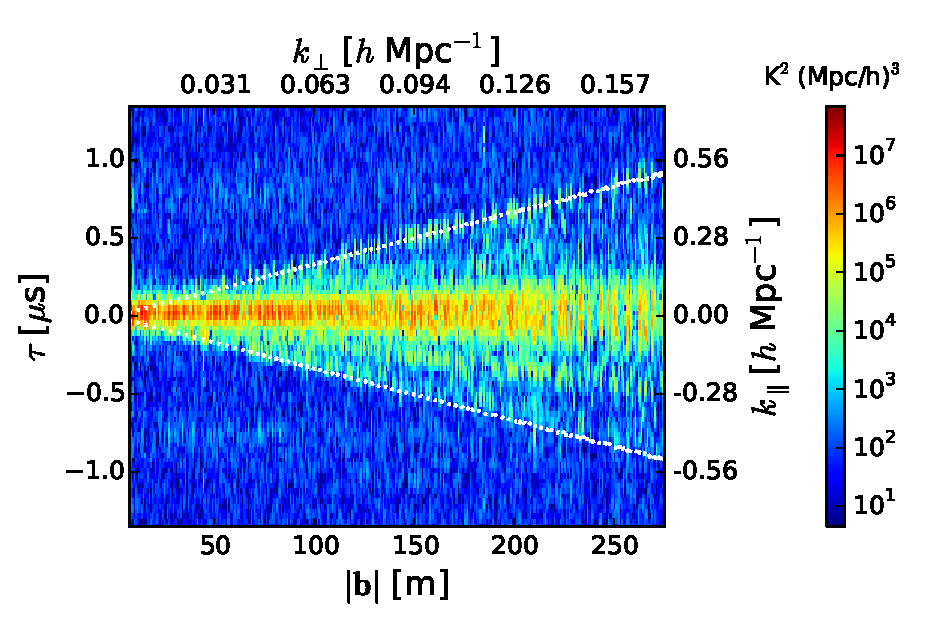
\includegraphics[width=\linewidth]{multi_baseline_CLEAN_fhd_avg_visibilities_amplitudes_185.0_MHz_30.7_MHz.eps}
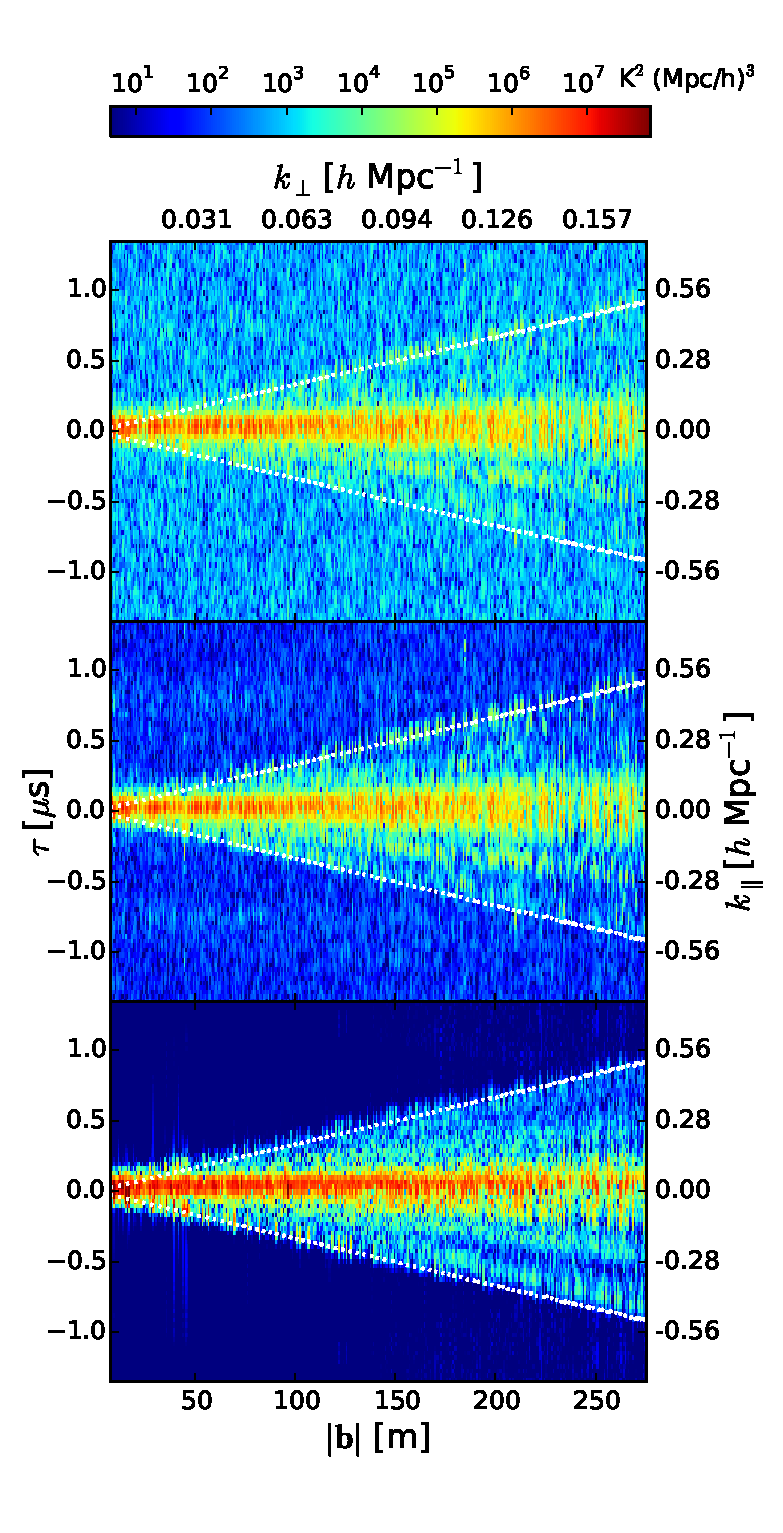
\includegraphics[width=\linewidth]{multi_baseline_fhd_sim_visibilities_amplitudes_comparison_185.0_MHz_30.7_MHz.eps}
\caption{Delay power spectra obtained from a single snapshot ({\it top}), by averaging 12 snapshots of LST aligned MWA data ({\it middle}), and from modeling with no thermal noise added ({\it bottom}). The $x$-axis, denoted by $|\boldsymbol{b}|$ (and $k_\perp$), represents angular (and spatial) scales in the plane of the sky while the $y$-axis, shown in $\tau$ and $k_\parallel$, denotes the spatial scales along the line of sight. White dotted lines are the horizon delay limits. Dynamic range in the delay power spectra of MWA data has increased by a factor $\sim 10$ after averaging (middle) relative to that in a single snapshot (top). Power near the horizon limits caused by wide-field effects are prominent. Faint horizontal features at $\tau=\pm 0.78\,\mu$s are visible due to effective lowering of thermal fluctuations and are the response to periodic coarse band edge flagging of MWA data every 1.28~MHz. \label{fig:delay-spectra}}
\end{figure}

The key defining feature of the {\it pitchfork} signature is an enhancement in foreground power near the horizon limits. In the individual snapshot, similar to the one used in our original study, faint features are visible near the horizon limits. But the high level of thermal fluctuations makes their significance marginal. In contrast, the dynamic range (in power spectrum units) in the averaged data (middle) is a factor $\gtrsim 10$ higher relative to that in a single snapshot (top), and is consistent with the improvement expected from averaging 12 independent snapshots. With this improvement in sensitivity, the foreground power near the horizon limits (white dotted lines) appears $\gtrsim 10$ times more prominent. We now note that faint horizontal features appear at $\tau = \pm 0.78\,\mu$s also as a result of lowering thermal fluctuations which is not seen in the single snapshot, thus confirming effective lowering of thermal fluctuations. We identify these faint features as the response in delay space of the MWA coarse band edges flagged periodically every 1.28~MHz. 

Figure~\ref{fig:3-baseline-comparison-delay-spectra} shows the averaged delay power spectra on three selected baseline vectors oriented northward. Data and noiseless models are shown in black and red respectively. The horizontal dotted black line denotes {\it rms} of thermal fluctuations estimated from data. The vertical dashed line denotes horizon delay limits, and the vertical dot-dashed lines denote delays at which the responses to coarse band edge flagging are expected.

\begin{figure}[htb]
\centering
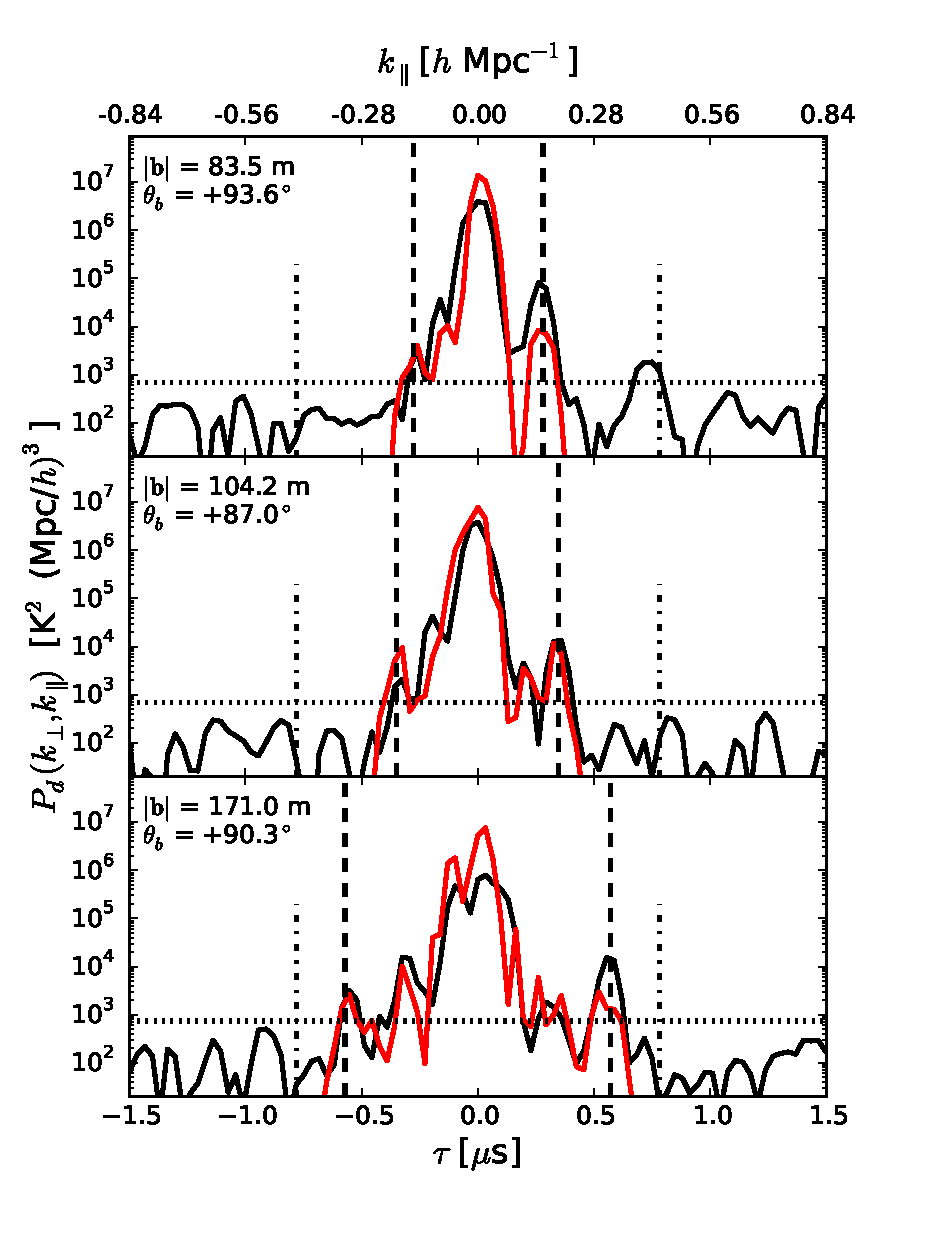
\includegraphics[width=\linewidth]{3_baseline_comparison_CLEAN_fhd_avg_visibilities_amplitudes_185.0_MHz_30.7_MHz.eps}
\caption{Delay power spectra on three antenna spacings oriented northward, obtained by coherent averaging of 12 snapshots aligned in LST. The averaged data and models are shown in black and red respectively. The antenna spacings are 83.5~m ({\it top}), 104.2~m ({\it middle}), and 171~m ({\it bottom}). The horizontal dotted line is the {\it rms} of thermal fluctuations. The vertical dashed lines denote the horizon delay limits. The vertical dot-dashed lines at $\tau=\pm 0.78\,\mu$s correspond to grating responses of periodic flagging of bandpass at intervals of 1.28~MHz. The peaks close to the horizon delay limits are distinctly visible at $\sim 10$-1000~$\sigma$ levels. Differences between model and data are primarily attributed to uncertainties in the foreground model and the MWA tile power pattern. \label{fig:3-baseline-comparison-delay-spectra}}
\end{figure}

The delay power spectra morphologies from data and modeling are remarkably similar in broad shape although they exhibit some differences in the amplitude scales. We attribute these differences to uncertainties in the foreground model, the MWA tile power pattern, thermal fluctuations, and other uncertainties noted in \citet{thy15}. 

We focus on the peaks near the horizon limits in the data. Typically, the power near the negative horizon limit is seen with a signal-noise ratio (SNR) $\sim$~10-100, while that around the positive horizon limit is $\sim$~100-1000. % The models of \citet{thy15} have noted that the foreground power near the horizon limits is due to the nature of wide-field measurements, and is predominantly composed of diffuse emission especially on baseline lengths $\lesssim 100$~m. 
Based on the morphological agreement between the data and the models, we conclude the features noted in our current analysis are a robust detection of the {\it pitchfork} signature predicted in our earlier study.

\section{Summary}\label{sec:summary}

Using deeper MWA data, we have confirmed with high significance the earlier prediction that wide-field EoR measurements suffer significant foreground contamination from near the horizon. This has important implications for instrument design and data analysis of future instruments such as HERA and SKA. 

Precise modeling is thus required to gain a complete understanding of the characteristics of the cosmological signal and the foregrounds. All-sky surveys matching the frequency and angular resolution of observation, and a detailed model of the instrument will further improve the accuracy of our models. In our earlier study, we proposed a selective flagging of data on different antenna spacings that can potentially mitigate foreground contamination by two orders of magnitude. Efforts are underway to incorporate this proposed foreground mitigation technique into the MWA data analysis algorithms.

For future work, we plan to extend our analysis to the upcoming instrument, HERA, which is currently under construction. It is a closely packed hexagonal array of fixed 14~m dishes which will observe the sky drifting overhead with redundant antenna spacings. Based on our earlier study, such a dish will have a much desirable Fourier response from a foreground contamination viewpoint. One of our objectives is to forecast the per-baseline foreground contamination as a function of local sidereal time in order to tune the observing strategy and data analysis to maximize sensitivity to the EoR signal.

% Fluctuations of redshifted H~{\sc i} from the reionization epoch are extremely faint relative to the radio foregrounds. This poses perhaps the greatest challenge to EoR experiments and thus merits a detailed characterization in order to separate them from the desired cosmological H~{\sc i} signal. 

% In a recent study, through the use of all-sky foreground and instrument models, the role of wide-field nature of radio interferometric measurements, hitherto unpredicted, has emerged. Referred to as the {\it pitchfork} signature in the delay spectral domain, it is characterized by significant foreground power in the primary field of view and an enhancement in power near the horizon. The latter is due to the highly nonlinear mapping between geometric delays and subtended solid angles, besides an increase in sensitivity to larger scales caused by foreshortening of baseline lengths along these directions. Owing to its localization in the delay domain, it is a leading cause of contamination in Fourier modes most sensitive to the EoR H~{\sc i} signal. 

% Knowledge of these characteristics weigh heavily on choices in instrument design like antenna aperture and in data analysis such as optimal weighting schemes for future instruments such as HERA and SKA. We report the first robust detection of the {\it pitchfork} signature (which could not be confirmed earlier in single MWA snapshots due to large thermal fluctuations) with a signal-noise ratio $>10$ made possible by coherent averaging of 12 independent LST-aligned snapshots from MWA observations. 

\acknowledgments

This work was supported by the U. S. National Science Foundation (NSF) through award AST-1109257. DCJ is supported by an NSF Astronomy and Astrophysics Postdoctoral Fellowship under award AST-1401708. JCP is supported by an NSF Astronomy and Astrophysics Fellowship under award AST-1302774. This work makes use of the Murchison Radio-astronomy Observatory, operated by CSIRO. We acknowledge the Wajarri Yamatji people as the traditional owners of the Observatory site. Support for the MWA comes from the NSF (awards: AST-0457585, PHY-0835713, CAREER-0847753, and AST-0908884), the Australian Research Council (LIEF grants LE0775621 and LE0882938), the U.S. Air Force Office of Scientific Research (grant FA9550-0510247), and the Centre for All-sky Astrophysics (an Australian Research Council Centre of Excellence funded by grant CE110001020). Support is also provided by the Smithsonian Astrophysical Observatory, the MIT School of Science, the Raman Research Institute, the Australian National University, and the Victoria University of Wellington (via grant MED-E1799 from the New Zealand Ministry of Economic Development and an IBM Shared University Research Grant). The Australian Federal government provides additional support via the Commonwealth Scientific and Industrial Research Organisation (CSIRO), National Collaborative Research Infrastructure Strategy, Education Investment Fund, and the Australia India Strategic Research Fund, and Astronomy Australia Limited, under contract to Curtin University. We acknowledge the iVEC Petabyte Data Store, the Initiative in Innovative Computing and the CUDA Center for Excellence sponsored by NVIDIA at Harvard University, and the International Centre for Radio Astronomy Research (ICRAR), a Joint Venture of Curtin University and The University of Western Australia, funded by the Western Australian State government.  

% \par\bigskip
\bibliographystyle{apj}
\bibliography{eor}

\end{document}
